\documentclass[../Main.tex]{subfiles}

\definecolor{codegreen}{rgb}{0,0.6,0}
\definecolor{codegray}{rgb}{0.5,0.5,0.5}
\definecolor{codepurple}{rgb}{0.58,0,0.82}
\definecolor{backcolour}{rgb}{0.95,0.95,0.92}

\lstdefinestyle{mystyle}{
    backgroundcolor=\color{backcolour},   
    commentstyle=\color{codegreen},
    keywordstyle=\color{magenta},
    numberstyle=\tiny\color{codegray},
    stringstyle=\color{codepurple},
    basicstyle=\ttfamily\footnotesize,
    breakatwhitespace=false,         
    breaklines=true,                 
    captionpos=b,                    
    keepspaces=true,                 
    numbers=left,                    
    numbersep=5pt,                  
    showspaces=false,                
    showstringspaces=false,
    showtabs=false,                  
    tabsize=2
}

\lstset{style=mystyle}
\begin{document}

    \section{Pruebas unitarias}
    \subsection{Descripción}
    \begin{justify}
    Las pruebas unitarias o unit testing lo que busca es corroborar el comportamiento correcto de una unidad de código.
    
    Django proporciona un framework de pruebas con una pequeña jerarquía de clases que se basan en la librería unittest estándar Python, esta librería es adecuada tanto para pruebas unitarias como pruebas de integración, en el backend del prototipo web GQuestions se hicieron pruebas unitarias.  
    
    Django ofrece métodos y herramientas que ayudan a probar el comportamiento, estos permiten simular las solicitudes con inserción de datos de prueba e inspección de la respuesta a las solicitudes.
    
    Para escribir pruebas existen clases base de prueba de Django como SimpleTestCase, TransactionTestCase, TestCase, LiveServerTestCase. En el backend se realizaron pruebas utilizando la clase base \textbf{TestCase}, se escribieron métodos por separado para verificar que los modelos del proyecto que hacen parte del diseño propio no tuviesen errores.
    
    \subsection{Detalles}
    Se probó aspectos del código escrito respecto a los modelos (base de datos) más no de bibliotecas o funcionalidades proporcionadas por Python o Django. Estos aspectos fueron el texto utilizado para etiquetas (atributos), tamaños de campos asignados y valores por defecto asignados.
    
    A continuación, se presentas algunos casos de prueba y posteriormente una descripción general de la creación de estas pruebas en Django utilizando TestCase.
    \end{justify}
    
    \begin{table}[H]
	\begin{Center}
		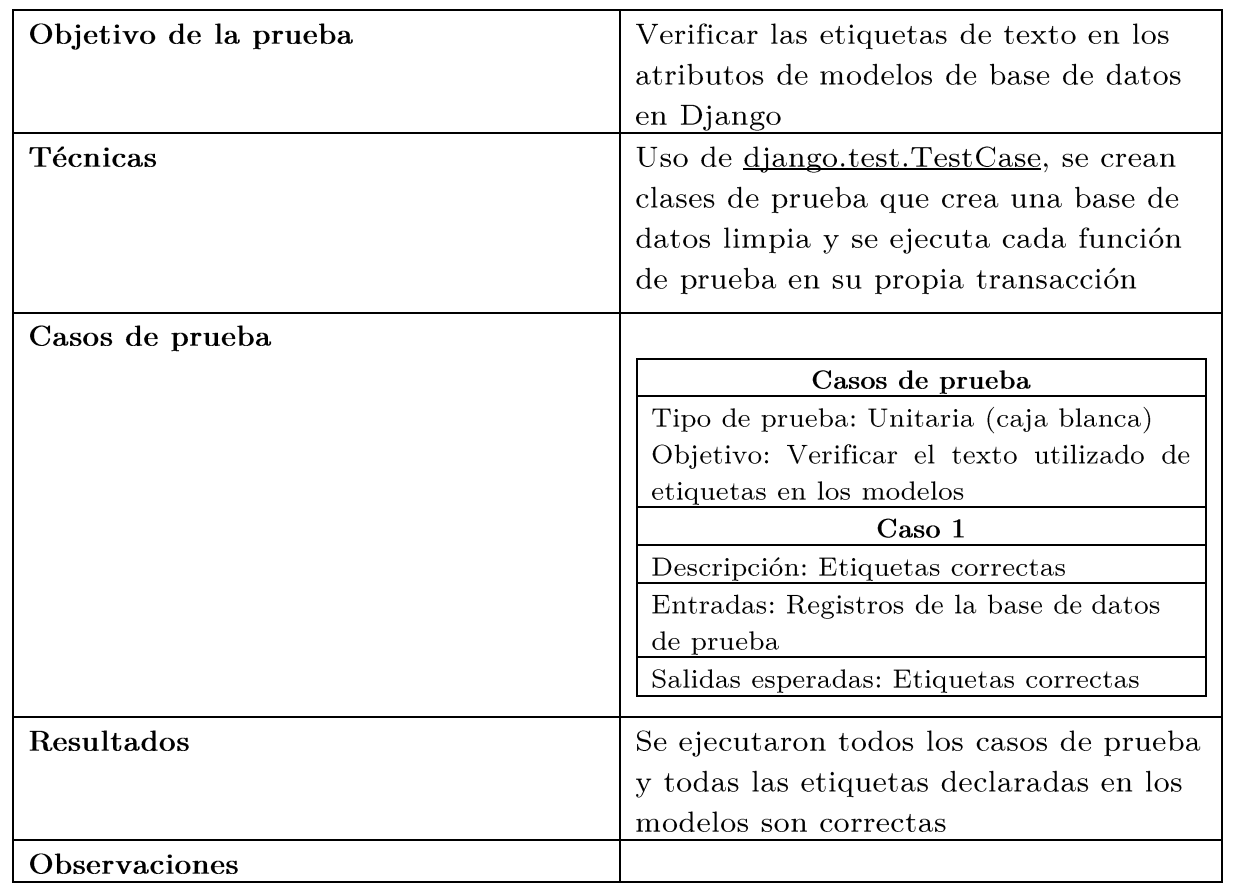
\includegraphics[width=5.8in,height=4.2in]{Chapters/06ChapterPruebas/images/caso_prueba_django.png}
	    \caption{Caso de prueba etiquetas de campos}
	    Fuente: Elaboración propia
        \label{tab:table1}
	\end{Center}
    \end{table}

    Uno de los modelos del Backend es la tabla \textbf{\texttt{Generación}} definida en Django, utilizando este modelo de ejemplo, se probó las etiquetas de todos los campos (ej. \texttt{\textbf{n\_examenes} = models.SmallIntegerField(null=False)}), porque a pesar de no haberse especificado explícitamente la mayoría, se tiene un diseño que dice cuáles deben ser estos valores. Si no se prueban lo valores, entonces no se sabe si las etiquetas de los campos tienen efectivamente los valores deseados. De esta manera, sucede lo mismo con las longitudes de campo específicadas (max\_length) y valores de campo por defecto (\texttt{ej. inicio\_oracion = models.CharField(max\_length=30, null=False, default='Aleatorio')}).
    
    Para probar el modelo se comienza por crear una clase \texttt{GeneracionModelTest} que recibe como argumento \texttt{TestCase}. Se escribe un método de clase \texttt{setUpTestData} que permite la creación de datos de prueba iniciales 
    (\texttt{ej. GeneracionModel.objects.create(id='ff6eb8f3' , n\_examenes=10,  n\_preguntas=5, account)}).
    
    Una vez se tiene el método de clase \texttt{setUpTestData} se escriben los métodos de clase de pruebas, para esto se utiliza los \texttt{Assert} que ofrece TestCase para comparar la etiqueta del campo deseada con la que trae de la base de datos; en este caso se verifica que el campo tenga el valor de etiqueta de campo correcta \texttt{verbose\_name}, de manera similar se escribieron los pruebas de tamaño de campo y de valores por defecto.
    
    Todos los modelos creados en Django fueron probados de la forma anteriormente expuesta (pruebas unitarias).

\end{document}

